\documentclass[11pt]{article}
\usepackage{listings}
\usepackage{tikz}
\usepackage{url}
\usepackage{hyperref}
%\usepackage{algorithm2e}
\usetikzlibrary{arrows,automata,shapes,positioning}
\tikzstyle{block} = [rectangle, draw, fill=blue!20, 
    text width=2.5em, text centered, rounded corners, minimum height=2em]
\tikzstyle{bw} = [rectangle, draw, fill=blue!20, 
    text width=3.5em, text centered, rounded corners, minimum height=2em]

\newcommand{\handout}[5]{
  \noindent
  \begin{center}
  \framebox{
    \vbox{
      \hbox to 5.78in { {\bf ECE459: Programming for Performance } \hfill #2 }
      \vspace{4mm}
      \hbox to 5.78in { {\Large \hfill #5  \hfill} }
      \vspace{2mm}
      \hbox to 5.78in { {\em #3 \hfill #4} }
    }
  }
  \end{center}
  \vspace*{4mm}
}

\lstset{basicstyle=\ttfamily \scriptsize}

\newcommand{\lecture}[4]{\handout{#1}{#2}{#3}{#4}{Lecture #1}}
\topmargin 0pt
\advance \topmargin by -\headheight
\advance \topmargin by -\headsep
\textheight 8.9in
\oddsidemargin 0pt
\evensidemargin \oddsidemargin
\marginparwidth 0.5in
\textwidth 6.5in

\parindent 0in
\parskip 1.5ex
%\renewcommand{\baselinestretch}{1.25}

% http://gurmeet.net/2008/09/20/latex-tips-n-tricks-for-conference-papers/
\newcommand{\squishlist}{
 \begin{list}{$\bullet$}
  { \setlength{\itemsep}{0pt}
     \setlength{\parsep}{3pt}
     \setlength{\topsep}{3pt}
     \setlength{\partopsep}{0pt}
     \setlength{\leftmargin}{1.5em}
     \setlength{\labelwidth}{1em}
     \setlength{\labelsep}{0.5em} } }
\newcommand{\squishlisttwo}{
 \begin{list}{$\bullet$}
  { \setlength{\itemsep}{0pt}
     \setlength{\parsep}{0pt}
    \setlength{\topsep}{0pt}
    \setlength{\partopsep}{0pt}
    \setlength{\leftmargin}{2em}
    \setlength{\labelwidth}{1.5em}
    \setlength{\labelsep}{0.5em} } }
\newcommand{\squishend}{
\end{list}  }
\newtheorem{example}{Example}


\begin{document}

\lecture{13 --- February 2, 2015}{Winter 2015}{Patrick Lam}{version 1}
\subsection*{Value Speculation}
The other kind of speculation is value speculation. In this case,
there is a (true) dependency between the result of a computation 
and its successor:
% note: v1 is meant to be the result you get from longCalculation this time, while last_value is what you got last time. (The code doesn't show that). If you get the same result from longCalculation this time as you did last time, then secondLongCalculation is correct and you don't need to redo it.

{\small \begin{verbatim}
  void doWork(int x, int y) {
    int value = longCalculation(x, y);
    return secondLongCalculation(value);
  }
\end{verbatim} }
If the result of {\tt value} is predictable, then we can speculatively
execute {\tt secondLongCalculation} based on the predicted value.
(Most values in programs are indeed predictable).
{\small \begin{verbatim}
void doWork(int x, int y) {
    thread_t t1, t2;
    point p(x,y);
    int v1, v2, last_value;
    thread_create(&t1, NULL, &longCalculation, &p);
    thread_create(&t2, NULL, &secondLongCalculation,
                  &last_value);
    thread_join(t1, &v1);
    thread_join(t2, &v2);
    if (v1 == last_value) {
      return v2;
    } else {
      last_value = v1;
      return secondLongCalculation(v1);
    }
}
\end{verbatim}
}
Note that this is somewhat similar to memoization, except with 
parallelization thrown in. In this case, the original running time is
\[ T = T_1 + T_2, \]
while the speculatively parallelized code takes time
\[ T_s = \max(T_1, T_2) + S + pT_2,\]
where $S$ is still the synchronization overhead, and $p$ is the probability that
\verb+v1 != last_value+.

\paragraph{Exercise.} Do the same computation as for speculative execution.

\subsection*{When can we speculate?}
Speculation isn't always safe. We need the following conditions:
  \begin{itemize}
    \item {\tt longCalculation} and {\tt secondLongCalculation} must not call
      each other.
    \item {\tt secondLongCalculation} must not depend on
      any values set or modified by {\tt longCalculation}.
    \item The return value of {\tt longCalculation} must be deterministic.
  \end{itemize}

As a general warning: Consider the \emph{side effects} of function calls.

\section*{Critical Paths}
You should be familiar with the concept of a critical path from previous
courses; it is the minimum amount of time to complete the task, taking
dependencies into account, and without speculating.

Consider the following diagram, which illustrates dependencies between
tasks (shown on the arrows). 
Note that B depends on A, and D depends on B and C, but C does
not depend on anything, so it could be done in parallel with
everything else. You can also compute expected execution times
for different strategies.
\begin{center}
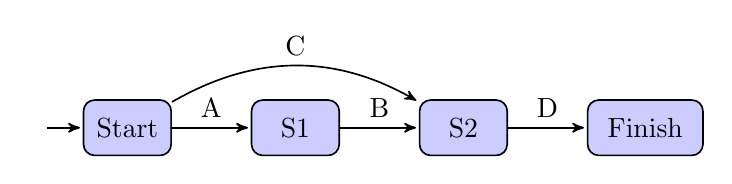
\begin{tikzpicture}[->,>=stealth',shorten >=1pt,auto,column sep=2.2cm,
                    semithick,initial text=]
  \node[initial,block] (s0) {Start};
  \node[block] (s1) [right=of s0] {S1};
  \node[block] (s2) [right=of s1] {S2};
  \node[bw] (s3) [right=of s2] {Finish};

  \path (s0) edge node {A} (s1)
        (s1) edge node {B} (s2)
        (s2) edge node {D} (s3)
        (s0) edge[bend left=30] node {C} (s2);
\end{tikzpicture}
\end{center}

\section*{Data and Task Parallelism}
There are two broad categories of paralellism: data parallelism and
task parallelism. An analogy to data parallelism is hiring a call
center to (incompetently) handle large volumes of support calls,
\emph{all in the same way}. Assembly lines are an analogy to task
parallelism: each worker does a \emph{different} thing.

More precisely, in data parallelism, multiple threads perform the
\emph{same} operation on separate data items. For instance, you have a
big array and want to double all of the elements. Assign part of the
array to each thread. Each thread does the same thing: double array
elements.

In task parallelism, multiple threads perform \emph{different}
operations on separate data items. So you might have a thread that
renders frames and a thread that compresses frames and combines them
into a single movie file.

We'll continue by looking at a number of parallelization patterns,
examples of how to apply them, and situations where they might apply.

\subsection*{Data Parallelism with SIMD}
We'll talk about single-instruction multiple-data (SIMD) later on in
this course, but here's a quick look. Each SIMD
instruction operates on an entire vector of data. These instructions
originated with supercomputers in the 70s. More recently, GPUs; the
x86 SSE instructions; the SPARC VIS instructions; and the
Power/PowerPC AltiVec instructions all implement SIMD.

\paragraph{Code.} Let's look at an application of SIMD instructions.

\begin{verbatim}
void vadd(double * restrict a, double * restrict b, int count) {
  for (int i = 0; i < count; i++)
    a[i] += b[i];
}
\end{verbatim}

Compiling this without SIMD on a 32-bit x86 ({\tt gcc -m32 -march=i386 -S}) might give this:
\begin{verbatim}
loop:
  fldl  (%edx)
  faddl (%ecx)
  fstpl (%edx)
  addl  8, %edx
  addl  8, %ecx
  addl  1, %esi
  cmp   %eax, %esi
  jle   loop
\end{verbatim}

We can instead compile to SIMD instructions ({\tt gcc -m32 -march=prescott -mfpmath=sse})
and get something like this:
\begin{verbatim}
loop:
  movupd (%edx),%xmm0
  movupd (%ecx),%xmm1
  addpd  %xmm1,%xmm0
  movpd  %xmm0,(%edx)
  addl   16,%edx
  addl   16,%ecx
  addl   2,%esi
  cmp    %eax,%esi
  jle    loop
\end{verbatim}
The \emph{packed} operations ({\tt p}) operate on multiple data
elements at a time (what kind of parallelism is this?)
The implication is that the loop only needs to loop half as many times.
Also, the instructions themselves are more efficient, because they're
not stack-based x87 instructions.

SIMD is different from the other types of parallelization we're
looking at, since there aren't multiple threads working at once.
It is complementary to using threads, and good for cases
where loops operate over vectors of data. These loops could also be
parallelized; multicore chips can do both, achieving high throughput.
SIMD instructions also work well on small data sets, where thread startup
cost is too high, while registers are just there to use.


\subsection*{Parallelization using Threads or Processes}
We'll be looking at thread-based or process-based parallelization for the
next bit. We don't care about the distinction between threads and processes
for the moment. In fact, we could even distribute work over multiple systems.

\paragraph{Pattern 1: Multiple Independent Tasks.} If you're just trying to maximize
system utilization, you can use one system to run a number of independent
tasks; for instance, you can put both a web server and database on
one machine. If the web server happens to be memory-bound while the
database is I/O-bound, then both can use system resources. If the web
server isn't talking to the database (rare these days!), then the tasks
would not get in each others' way.

Most services probably ought to be run under virtualization these
days, unless they're trivial or not mission-critical.

A more relevant example of multiple independent tasks occurs in
cluster/grid/cloud computing: the cloud might run a number of
independent tasks, and each node would run some of the tasks. The
cloud can retry a task (on a different node, perhaps) if it fails on
some node. Note that the performance ought to increase linearly with
the number of threads, since there shouldn't be communication between
the tasks.

\paragraph{Pattern 2: Multiple Loosely-Coupled Tasks.} Some applications contain
tasks which aren't quite independent (so there is some inter-task
communication), but not much.  In this case, the tasks may be
different from each other. The communication might be from the tasks
to a controller or status monitor; it would usually be asynchronous or
be limited to exceptional situations.

Refactoring an application this way can help with latency: if you 
split off the CPU-intensive computations into a sub-thread, then
the main thread can respond to user input more quickly.

Here's an example. Assume that an application needs to receive and
forward network packets, and also must log packet activity to disk.
Then the two tasks are clear: receive/forward, and log. Since logging
to disk is a high-latency event, a single-threaded application might
incur latency while writing to disk. Splitting into subtasks allows
the receive/forward to run without waiting for previous packets to be
logged, thus increasing the throughput of the system.

\paragraph{Pattern 3: Multiple Copies of the Same Task.} A common variant of
multiple independent tasks is multiple copies of the same task
(presumably on different data). In this case, we'd require there to be
no communication between the different copies, which would enable
linear speedup. An example is a rendering application running on
multiple distinct animations. We gain throughput, but need to wait
just as long for each task to complete.

\paragraph{Pattern 4: Single Task, Multiple Threads.} This is the classic
vision of ``parallelization'': for instance, distribute array
processing over multiple threads, and let each thread compute the
results for a subset of the array.

This pattern, unlike many of the others before it, can actually
decrease the time needed to complete a unit of work, since it gets
multiple threads involved in doing the single unit simultaneously.
The result is improved latency and therefore increased throughput.
Communication can be a problem, if the data is not nicely
array-structured, or has dependencies between different array parts.

Other names and variations for this pattern include ``fork-join'',
where the main process forks its execution and gives work to all of
the threads, with the join synchronizing threads and combining the
results; and ``divide-and-conquer'', where a thread spawns subthreads
to compute smaller and smaller parts of the solution.

\end{document}
